\section{Implementation}
\label{VT:Sec:Implementation}

The implementation of the virtual time system and its integration with Mininet-Hifi (the latest version of Mininet) is composed of three parts,
as shown in Figure~\ref{VT:Fig:VTMininetHifi}.
First, we built a lightweight and independent middleware in the Linux kernel to provide virtual time support to user-space software.
Second, we slightly modified the initialization procedure of Mininet with two additional python modules to realize (adaptive) virtual time in Mininet.
Third, we discuss our design to enable transparent support of virtual time for applications running in the containers.

\begin{figure}
\centering
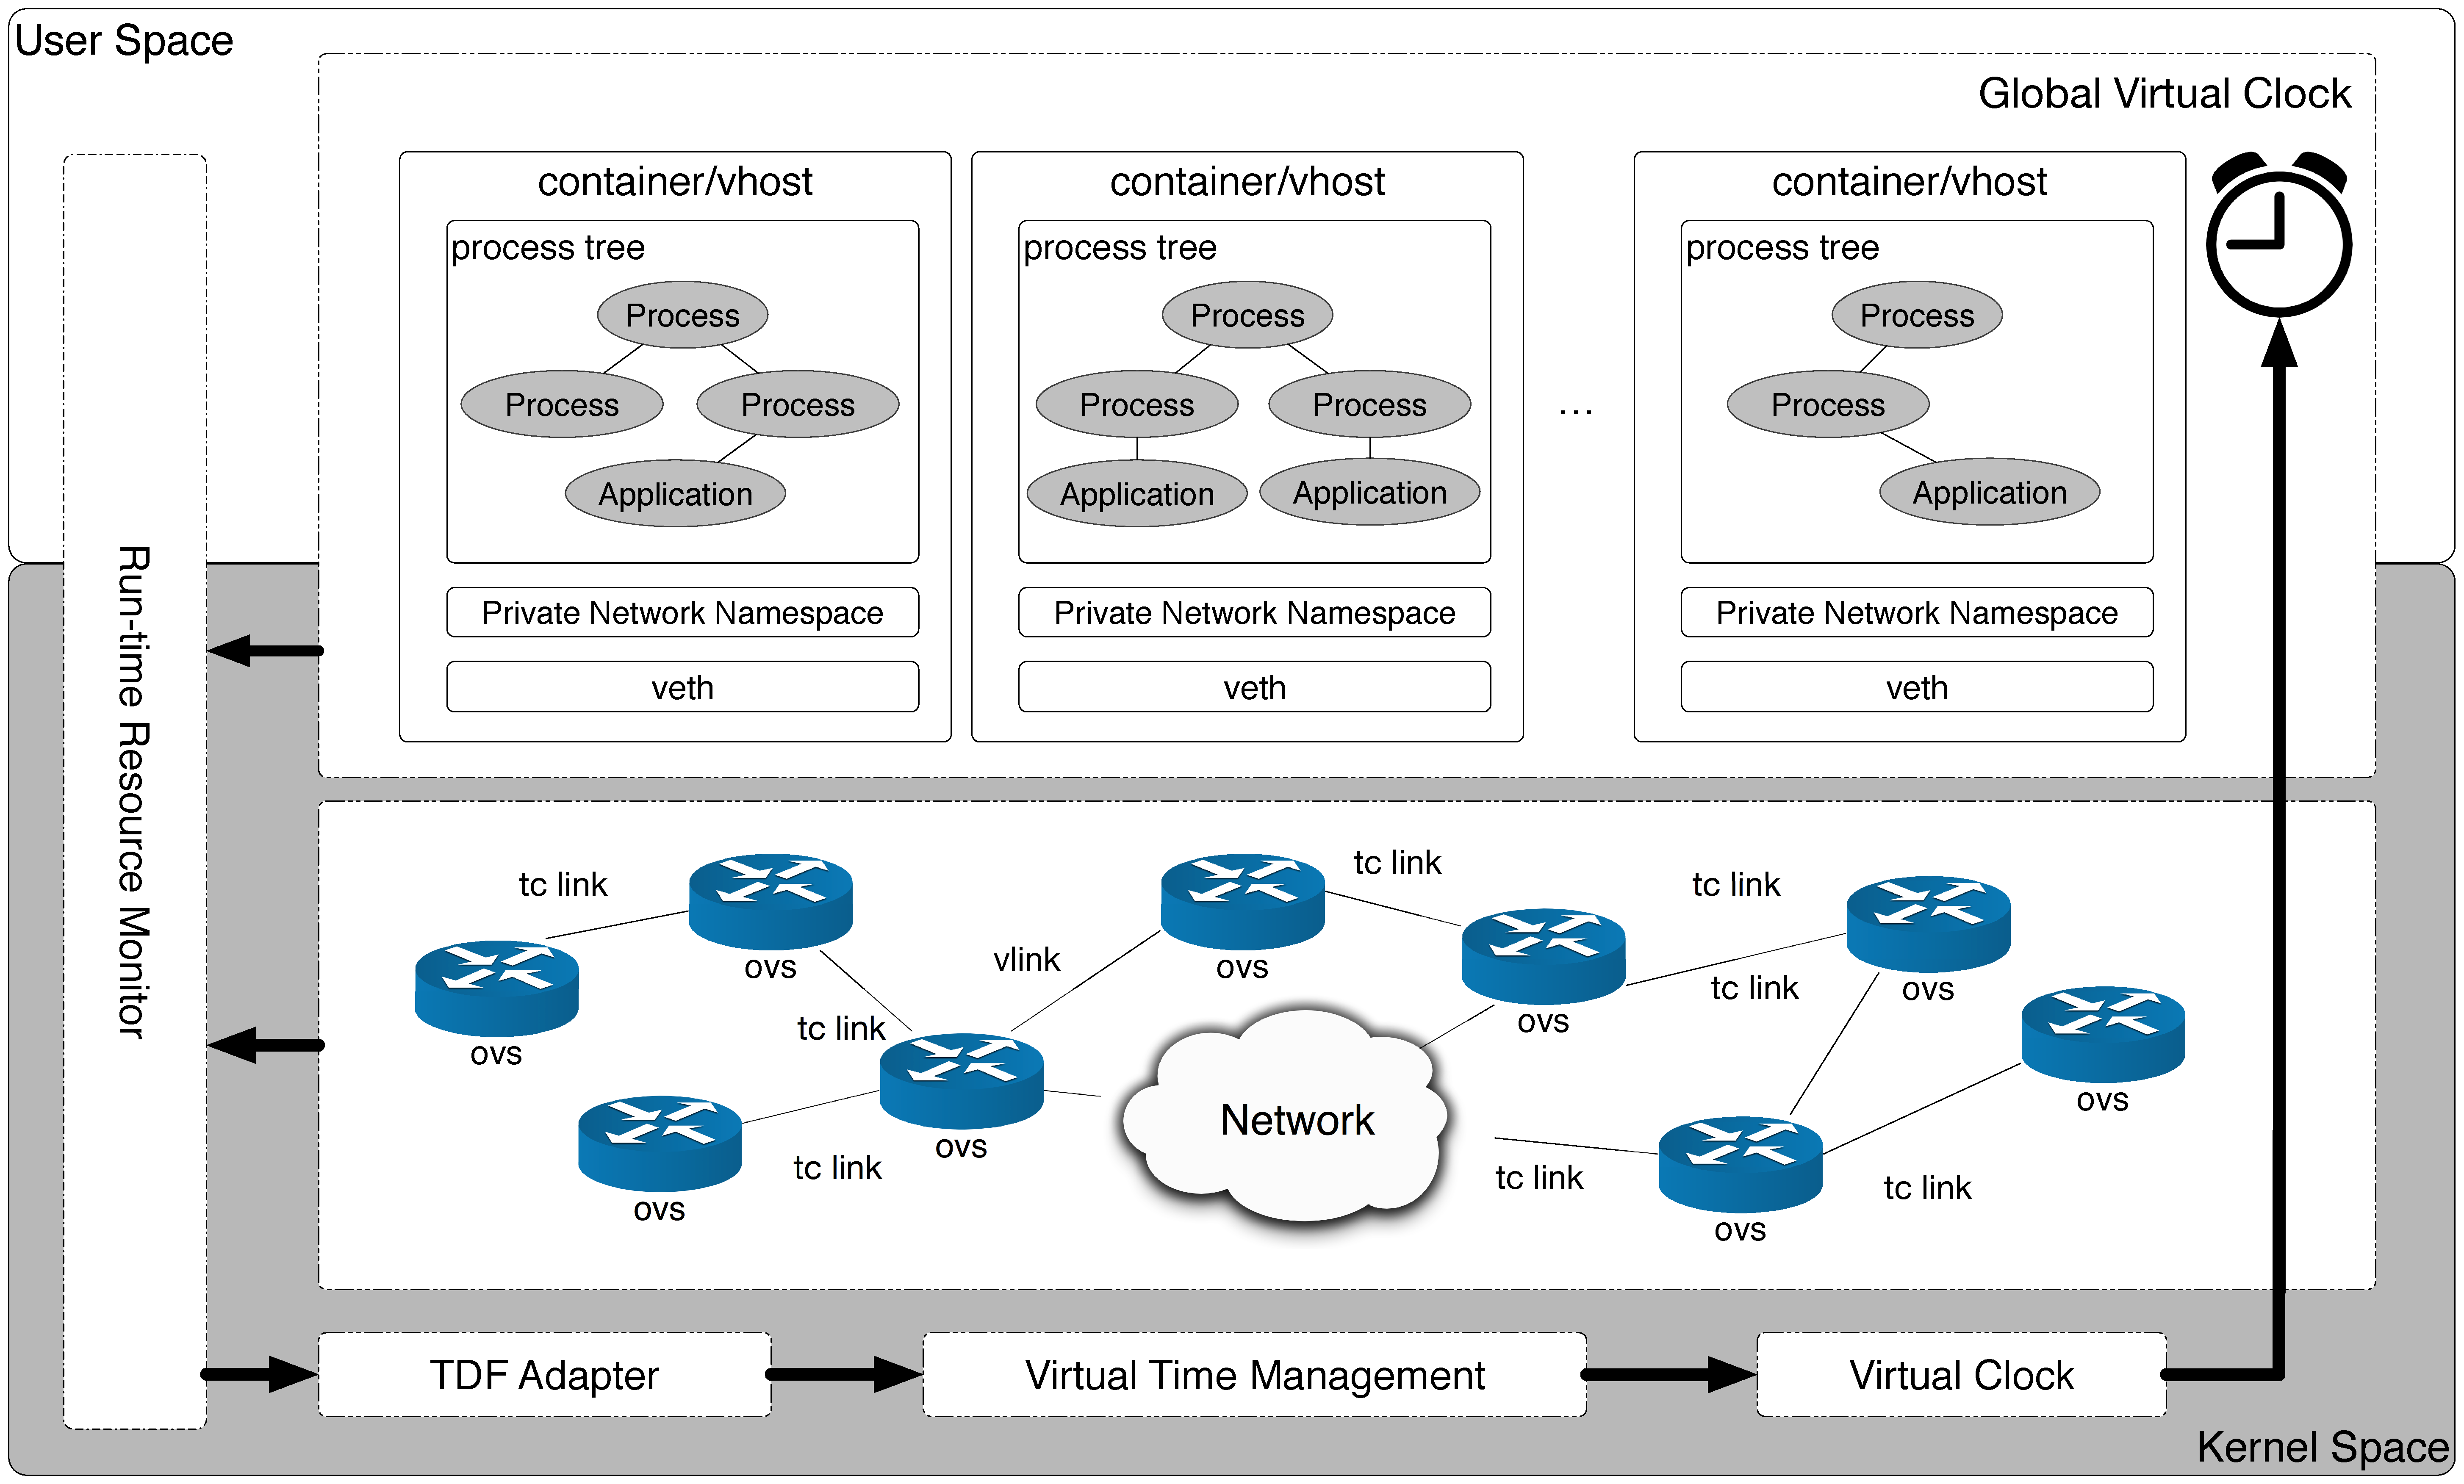
\epsfig{file=VirtualTime/figures/VT-Mininet-Hifi.eps, width=0.9\textwidth}
\caption{Integration of Mininet-Hifi and Virtual Time}
\label{VT:Fig:VTMininetHifi}
\end{figure}

\subsection{Modification in Linux Kernel}
\paragraphbe{Timing-related Kernel Modifications.}
\label{VT:SubSec:ExtendLinuxKernel}
Our implementation is based on a recent Linux kernel 3.16.3 with no third-part library dependency.
To make a process have its own perception of time, we added the following four new fields in the \texttt{task\_struct} struct type.
\begin{itemize}
    \item \texttt{physical\_start\_ns} represents the starting time that a process detaches from the system clock and begins to use the virtual time, in nanoseconds.
    \item \texttt{physical\_past\_nsec} represents how much physical time has elapsed since the last time the process requested the current time, in nanoseconds
    \item \texttt{virtual\_start\_nsec} represents the starting time that a process detaches from the system clock and uses the virtual time, in nanoseconds 
	\item \texttt{virtual\_past\_nsec} represents how much virtual time has elapsed since the last time the process requested the current time, in nanoseconds
    \item \texttt{freeze\_start\_ns} represents the starting time that a process or a process group is frozen. It is always zero for a non-frozen process.
    \item \texttt{freeze\_past\_ns} represents the cumulative time, in nanoseconds, that a running process or a process group remains in the frozen state.
	\item \texttt{dilation} represents the TDF of a time-dilated process
\end{itemize}

\begin{algorithm}[ht]
    \DontPrintSemicolon
    \KwIn{$tk = $ C struct \texttt{task\_struct} representing a process in Linux kernel \newline
    $dilation = $ value of time dilation factor}
    \SetKwProg{Fn}{Function}{}{\KwRet}
    \SetKwFunction{InitVT}{init\_virtual\_time}
    \SetKwFunction{GetNS}{getnstimeofday}
    \SetKwFunction{TSNS}{timespec\_to\_ns}
    \Fn{\InitVT{$tk$, $dilation$}} {
        \If {$dilation > 0$} {
            $tk.virtual\_start\_nsec \gets 0$ \;
            $ts \gets$ \GetNS{} \;
            $tk.virtual\_start\_nsec \gets$ \TSNS{$ts$} \;
            $tk.virtual\_past\_nsec \gets 0$ \;
            $tk.physical\_past\_nsec \gets 0$ \;
            $tk.dilation \gets dilation$
        }
    }
    \caption{Initialize Virtual Time}
    \label{VT:Alg:InitVirtualTime}
\end{algorithm}

\begin{algorithm}[ht]
    \DontPrintSemicolon
    \KwIn {$p = $ the current running process in Linux kernel \newline
    $ts = $ current wall clock time \newline
    $tdf = p.dilation$}
    \SetKwProg{Fn}{Function}{}{\KwRet}
    \SetKwFunction{UpdatePPN}{update\_physical\_past\_nsec}
    \SetKwFunction{UpdateVPN}{update\_virtual\_past\_nsec}
    \SetKwFunction{DoDilate}{do\_virtual\_timekeeping}
    \SetKwFunction{TSNS}{timespec\_to\_ns}
    \SetKwFunction{NSTS}{ns\_to\_timespec}
    \Fn{\UpdatePPN{$ts$}} {
        $now \gets \TSNS{$ts$}$ \;
        $delta\_ppn \gets now - p.physical\_past\_nsec - p.physical\_start\_nsec - p.freeze\_past\_nsec$ \;
        $p.physical\_past\_nsec += delta\_ppn$ \;
        \KwRet{$delta\_ppn$} \;
    }
    \Fn{\UpdateVPN{$delta\_ppn$}} {
        $delta\_vpn \gets 0$ \;
        \If {$tdf > 0$} {
            $delta\_vpn \gets delta\_ppn / tdf$ \;
            $p.virtual\_past\_nsec += delta\_vpn$ \;
        }
        \KwRet{$delta\_vpn$}
    }
    \Fn{\DoDilate{$ts$}} {
        \If {$p.virtual\_start\_ns > 0$} {
            $delta\_ppn \gets \UpdatePPN{ts}$ \;
            $delta\_vpn \gets \UpdateVPN{delta\_ppn, tdf}$ \;
            $virtual\_now = p.virtual\_start\_nsec + p.virtual\_past\_nsec$ \;
            $virtual\_ts = \NSTS{virtual\_now}$ \; 
            $ts.tv\_sec = virtual\_ts.tv\_sec$ \;
            $ts.tv\_nsec = virtual\_ts.tv\_nsec$ \;
        }
    }
    \caption{Virtual Timekeeping Algorithm}
    \label{VT:Alg:VirtualTimeKeeping}
\end{algorithm}

\begin{algorithm}
    \DontPrintSemicolon
    \KwIn {$tsk = $ the process/container in Linux kernel to be frozen or unfrozen}
    \SetKwProg{Fn}{Function}{}{\KwRet}
    \SetKwFunction{Freeze}{freeze}
    \SetKwFunction{Unfreeze}{unfreeze}
    \SetKwFunction{PopulateFreeze}{populate\_frozen\_time}
    \SetKwFunction{KillGroup}{kill\_pgrp}
    \SetKwFunction{TaskGroup}{task\_pgrp}
    \SetKwFunction{GetNS}{getnstimeofday}
    \SetKwFunction{TSNS}{timespec\_to\_ns}
    \Fn{\Freeze{tsk}} {
        \KillGroup{\TaskGroup{tsk}, \texttt{SIGSTOP}, 1} \;
        $ts = $\GetNS{} \;
        $tsk.freeze\_start\_nsec \gets$ \TSNS{ts} \;
    }
    \Fn{\PopulateFreeze{tsk}} {
        \ForEach {child $\in$ tsk.children} {
            $child.freeze\_past\_nsec \gets tsk.freeze\_past\_nsec$ \;
            \PopulateFreeze{child} \;
        }
    }
    \Fn{\Unfreeze{$tsk$}} {
        $ts = $\GetNS{} \;        
        $now \gets$ \TSNS{ts} \;
        $tsk.freeze\_past\_nsec += now - tsk.freeze\_start\_nsec$ \;
        $tsk.freeze\_start\_nsec \gets 0$ \;
        \PopulateFreeze{tsk} \;
        \KillGroup{\TaskGroup{$tsk$}, \texttt{SIGCONT}, 1} \;
    }
    \caption{Freeze and Unfreeze Linux Container}
    \label{VT:Alg:Freeze}
\end{algorithm}


Algorithm~\ref{VT:Alg:InitVirtualTime} and~\ref{VT:Alg:VirtualTimeKeeping} give the details about how we implement the time dilation. 
To preserve an accurate virtual clock in the kernel, we added a private function \texttt{do\_virtual\_timekeeping}
in the Linux's timekeeping subsystem to keep tracking the dilated virtual time based on the physical time passed and TDF. 
Based on process's \texttt{virtual\_start\_nsec}, the system determines the type of time to return, i.e., the physical system clock time or the virtual time.

\texttt{virtual\_start\_nsec} in \texttt{init\_virtual\_time} should first be initialized to zero so that the next \texttt{gettimeofday}
always returns the undilated time to compute and record the exact physical time that a process starts to use virtual time.
To return the accurate virtual time upon requests, the duration since the last call to \texttt{do\_virtual\_timekeeping} is calculated and precisely scaled with TDF. 
To enable virtual time support for a wide range of timing-related system calls,
we extensively traced the routines in Linux's subsystems that request timing information (such as \texttt{getnstimeofday},
\texttt{ktime\_get}, \texttt{ktime\_get\_ts}, etc.), and modified them to properly invoke \texttt{do\_virtual\_timekeeping}.

The algorithm to freeze/unfreeze processes is shown in Algorithm~\ref{VT:Alg:Freeze},
and is implemented in the Linux kernel.
After stopping a group of processes, we record the  current time for calculating the process frozen duration once we unfreeze the process.
Note that sending \texttt{SIGCONT} to all processes is behind the time keeping function.
The reason is that if we resume the process group first, an unfrozen process may be scheduled to run,
and possibly query time before we complete populating the \texttt{freeze\_past\_ns} within the entire container.
We also develop a user space utility program \texttt{freeze\_all\_proc}.
This program can freeze and unfreeze multiple hosts in parallel.
In particular, it spawns one \texttt{pthread} for every network host to write its freeze entry in the Proc system.
Since the network emulator always pauses or resumes all hosts, this optimization significantly reduces the running overhead in large-scale network settings.

The virtual file system provides an interface between the kernel and the user space.
Since virtual time is a per-process property, it is more efficient to create a \texttt{/proc}
file entry for the associated processes rather than adding system calls.
The virtual time interface consists of two extra file entries under \texttt{/proc/\$pid}.
\begin{itemize}
    \item \texttt{/proc/\$pid/dilation} A process \texttt{\$pid} can enable and disable virtual time, as well as change a new time dilation factor (TDF).
        To support fractional dilation values, a TDF of $x$ is stored in this entry as $1000x$,  since floating point numbers are rarely supported in the Linux kernel.
    \item \texttt{/proc/\$pid/freeze} We can freeze and unfreeze a process \texttt{\$pid} according to the written boolean value.
        A value 1 freezes the entire process group and a value 0 resumes all the processes in this group.
\end{itemize}

We make a distinction between regular processes and virtual-time enabled processes. In other words, the \texttt{/proc/\$pid/freeze} entry is only valid only if \texttt{/proc/\$pid/dilation}  already has a non-zero value. The emulator can enable a container with virtual time by writing 1000 to the \texttt{dilation} proc file entry. This will turn on the freeze/unfreeze capability without unnecessarily modifying the clock speed. In this work, we use a process calling system call \texttt{unshare()} with flag \texttt{CLONE\_NEWTIME} to enable virtual time.
This design is motivated and tailored to be compatible with Mininet's programming interface.
\paragraphbe{Process-related Kernel Modifications.}
To enable the virtual time perception to processes running in a network emulator, we added the following new system calls.
\begin{itemize}
    \item \texttt{virtualtimeunshare} is essentially the \texttt{unshare} system call with time dilation inputs.
        It is used by container-based emulators, such as Mininet, to create emulated nodes.
        \texttt{virtualtimeunshare} creates a new process with a TDF in a different \texttt{namespace} of its parent process according to \texttt{flags}.
    \item \texttt{settimedilaitonfactor} offers an interface to change the TDF of a process.
        Note that a command executed in an emulated host is equivalent to forking a shell command executed by \texttt{bash}. 
        Therefore, adjusting a process' TDF requires the change of the calling process' parent (e.g., host's \texttt{bash}),
        which occasionally would lead to tracing back to the root of the process tree, especially in the case of dynamic TDF adjustment. 
\end{itemize}

We also modified the \texttt{do\_fork} system call to initialize the virtual-time-related attributes of a process,
such as using the variable \texttt{stack\_size} to pass the TDF value. 
Another option is to set TDF to a default value in \texttt{virtualtimeunshare} and
then relies on explicitly invoking \texttt{settimedilationfactor} to set desired TDF;
this method prevents modifying the interface of creating \texttt{namespace} in traditional Linux. 
Functions in \texttt{timekeeping.c} were modified to invoke \texttt{do\_dilatetimeofday}
in order to return the virtual time to system calls like \texttt{gettimeofday} and other kernel routines that request timing information.


\paragraphbe{Networking-related Kernel Modifications.}
In this work, we focus on capturing all the related system calls and kernel routings to support virtual time in Linux container with the application of Mininet. 
One particular case related to Mininet is the usage of \texttt{tc}, a network quality-of-service control module in Linux~\cite{TrafficControl}. 
For instance, we can use \texttt{tc} to rate-limit a link to 100 Mbps using Hierarchic Token Bucket (HTB) \texttt{qdisc} in Mininet. If the TDF is set to 8, the link bandwidth would be approximately 800 Mbps from the emulated hosts' viewpoints as we observed from the time-dilated \texttt{iperf3} application.

As a network module in Linux, \texttt{tc} does not reference Linux kernel's time as the way user application does. 
Therefore, \texttt{tc} is transparent to our virtual time system. One way to solve this problem is to modify the network scheduling code in kernel to provide \texttt{tc} with a dilated traffic rate. 
In the earlier example with TDF set to 8, the experiment will run 8 times slower than the real time, and we can configure \texttt{tc}'s rate limit as $rate/TDF=12.5$ Mbps to emulate a 100 Mbps link. 
Note that we only tailored HTB in \texttt{tc}, which is the default \texttt{qdisc} used by Mininet. 
We will generalize the mechanism to other \texttt{qdiscs} including HFSC (Hierarchical Fair Service Curve) and TBF (Token Bucket Filter) in the future.

\subsection{Modification in Network Emulator}
\paragraphbe{Virtual-Time-Enabled Mininet.}
\label{VT:SubSec:ImplementMininet}
%Mininet uses Linux's container \cite{LXC} to enable scalable network emulation. 
Containers allow groups of process running on the same kernel to have independent views of system resources, such as process IDs, file systems and network interfaces. 
We add the virtual time property to a container's \texttt{namespace}~\cite{LinuxNamespace} so that every container can have its own virtual clock. 
We design our system in the way that minimal modifications of Mininet are needed for integration, so that the virtual time system can be easily extended to other Linux-container-based applications. 

We modified the initialization procedure of Mininet, in particular, the \texttt{mnexec} program in Mininet, to process two additional parameters. 
When we create \texttt{Node}s in Mininet (hosts, switches, and controllers are all inherited from \texttt{Node}), users can feed in a TDF argument with \texttt{virtualtimeunshare} (as a replacement of \texttt{unshare}) with \texttt{-n} option. 
This way, a system-wide TDF can be conveniently set for all the emulated hosts. We also provide the ability to dynamically adjust the TDF for every emulated host during runtime. 
To do that, we added a new option \texttt{-t} in \texttt{mnexec} to invoke the aforementioned system call \texttt{settimedilaitonfactor} to do the actual TDF adjustment. 
The two modifications enable the integration of virtual time in Mininet, and also serve as the basis of the adaptive TDF management.

\paragraphbe{Adaptive TDF Scheduling.}
To optimize the performance of the virtual-time-enabled Mininet, we developed an adaptive TDF scheduler
through two python modules \texttt{MininetMonitor} and \texttt{DilationAdaptor}
(refer to Emulation Monitor and Time Dilation Adaptor in Figure~\ref{VT:Fig:ContainerVirtualTime})
to accelerate the experiment speed while preserving high fidelity.

\texttt{MininetMonitor} is responsible to monitor the CPU usage of the entire emulation system,
consisting of a group of processes including the Mininet emulator, the Open vSwitch module, and emulated nodes (e.g., SDN controllers, hosts and switches). 
Also, applications are dynamically created, executed and destroyed within containers, in the form of child processes of their parent containers. 
\texttt{MininetMonitor} utilizes the \texttt{ps} command to collect the group's aggregate CPU percentage
and periodically computes and passes the average CPU load statistics to \texttt{DilationAdaptor}. 
The core of \texttt{DilationAdaptor} is an adaptive algorithm to calculate an appropriate \textit{TDF}.
%Only after receiving a new \textit{TDF} can Mininet pause the experiment and update its global time dilation factor. Otherwise it enters the next Epoch directly. 
Global \textit{TDF} updating was achieved by invoking the \texttt{mnexec\ -t\ tdf} program for every running host. 


% Algorithm \ref{Alg-AdaptiveTDF} illustrates our adaptive TDF scheduling, and we implemented it as a threshold-based \texttt{DilationAdaptor}. 
% %From the input fed by \texttt{MininetMonitor}, \texttt{DilationAdaptor} first define current load status. The key idea here is: if emulator is overloaded, we increase TDF with a large value; if it is underloaded, we may consider decrease TDF with a large value. 

% \algnewcommand\algorithmicswitch{\textbf{switch}}
% \algnewcommand\algorithmiccase{\textbf{case}}
% \algnewcommand\algorithmicassert{\texttt{assert}}
% \algnewcommand\Assert[1]{\State \algorithmicassert(#1)}%
% % New "environments"
% \algdef{SE}[SWITCH]{Switch}{EndSwitch}[1]{\algorithmicswitch\ #1\ \algorithmicdo}{\algorithmicend\ \algorithmicswitch}%
% \algdef{SE}[CASE]{Case}{EndCase}[1]{\algorithmiccase\ #1}{\algorithmicend\ \algorithmiccase}%
% \algtext*{EndSwitch}%
% \algtext*{EndCase}%

% \algrenewcommand{\algorithmiccomment}[1]{\hskip1em$/*$ #1 $*/$}
% \begin{algorithm}
% \caption{Adaptive Time Dilation Factor Scheduling}\label{Alg-AdaptiveTDF}
% \begin{algorithmic}[1]
% \State{Decide emulation $state$ through the resource indicator}\Comment{e.g., CPU utilization}
% \State{$MAX$ denotes the maximum allowed TDF value.}
% \State{$\Delta_{large}, \Delta_{small}$ denote the customizable large and small adjustment}
% \Switch{$state$}
% 	\Case{$OVERLOADED$}
% 		\State{$TDF_{new}=TDF_{prev}+\Delta_{large}$}
% 	\EndCase
% 	\Case{$WARNING$}
% 		\State{$TDF_{new}=TDF_{prev}+\Delta_{small}*2$}
% 	\EndCase
% 	\Case{$MODERATE$}
% 		\If{$TDF_{prev} == MAX$}
% 			\State{$TDF_{new}=TDF_{prev}-\Delta_{large}$}
% 		\ElsIf{$TDF_{prev} > \Delta_{small}$}
% 			\State{$TDF_{new}=TDF_{prev}-\Delta_{small}$}
% 		\Else
% 			\State{$TDF_{new}=TDF_{prev}$}%\Comment{Do not change TDF}
% 		\EndIf
% 	\EndCase
% 	\Case{$LIGHT$}
% 		\If{$TDF_{prev} > \Delta_{large}*2$}
% 			\State{$TDF_{new}=TDF_{prev}-\Delta_{large}$}
% 		\Else
% 			\State{$TDF_{new}=TDF_{prev}-\Delta_{small}*2$}
% 		\EndIf
% 	\EndCase
% \EndSwitch
% %\State{return $TDF_{new}$}
% \end{algorithmic}
% \end{algorithm}

Our adaptive virtual time scheduling design is similar to the one used in~\cite{NtwkEmultAdaptVirtTime} in spirit with two major differences. 
First, both techniques target on different platforms. 
Our technique is applied to Linux-container-based network emulation to support scalable SDN experiments,
and theirs uses virtual routing and executes OpenVZ instances inside Xen. 
Second, their solution needs be deployed on a cluster to emulate a medium-scale network, which results in much higher communication overhead in two types:
(1) every VM's monitor needs to report the CPU usage, and
(2) the adaptor needs to send new TDF to every VM. 
Therefore, the message transmission delay in LAN and the processing delay in protocol stacks contributes to the overall communication delay. 
In contrast, \texttt{MininetMonitor} runs as a lightweight background thread in Mininet,
and \texttt{DilationAdaptor} is simply a python object that Mininet has a reference to. 
The communication in our system is through synchronized queues and method invocations, which is much faster. 

\subsection{Virtual Time Support for Network Applications}
\label{VT:SubSec:ModificationApplications}
Network applications running inside containers (e.g., \texttt{iperf3}~\cite{iperf3} or \texttt{ping}) should also use virtual time. 
We do not need to modify the application code because they are running as child processes of Mininet's hosts. 
A child process always copies its parent's \texttt{task\_struct} when it is forked including the same \texttt{dilation} and \texttt{virtual\_start\_nsec} values. 
Although \texttt{virtual\_start\_nsec} does not present the virtual starting time of the child process,
our algorithm is designed to work with relative values since it does necessary initial processes during \texttt{do\_fork}. 
When applications inquire about the system time,
the modified kernel knows that they are using virtual clock and return the virtual clock time instead of the system clock time.

One issue we notice is that the 64-bit Linux kernel running on Intel-based architectures provides the Virtual Dynamic Shared Object (vDSO)
and the \texttt{vsyscall} mechanism to reduce the overhead of context switches caused by the frequently invoked system calls,
for example, \texttt{gettimeofday} and \texttt{time}~\cite{VDSO}. 
Therefore, applications may bypass our virtual-time-based system calls unless we explicitly use the \texttt{syscall} function.
Our solution is to disable vDSO with respect to \texttt{\_\_vdso\_gettimeofday} in order to transparently offer virtual time to applications in the containers.
